\clearpage

\def\chaptertitle{Preliminaries}

\lhead{\emph{\chaptertitle}}

\chapter{\chaptertitle}
\label{ch:preliminaries}

\section{Analysis of Algorithms}
\label{sec:anaylsis-of-algorithms}

\subsection{Word-RAM Model \& Big Oh Notation}
Under the Word-RAM model there are four atomic operations that a CPU can perform: 
\begin{itemize}
    \item \textbf{Regiser (Re-)Initialization}: Set the content of a register to a fixed value, or to the content of another register.
    \item \textbf{Arithmetic Operations}: Take two integers $a$ and $b$ stored in two registers, calculate the following and then store the result in a register
    \item \textbf{Comparison and Branching}: Compare two integers $a$ and $b$ stored in two registers and decide which of the following is true: $a<b, a=b$ abd $a>b$
    \item \textbf{Memory Access}: Take the memory address $p$ stored in a register, then perform one of a read or write operation at adress $p$
\end{itemize}

Every algorithm can be viewed as a sequence of these four atomic operations. The \textit{running time cost} of an algorithm is the measured by the number of operations in the sequence, as a function of the size of the input $n$. The \textit{space consumption} of an algorithm is the measured by the footprint of memory cells which it touches, that is, the peak memory usage when the algorithm is running. We will commonly describe the growth of said function in terms of their Big-$O$, Big-$\Omega$ and Big-$\Theta$ complexity defined as follows

\begin{definition}[Big-$O$ Notation]
    We say $f(n)$ grows asymptotically no faster than $g(n)$ if there exists two positive constants $c_1$ and $c_2$ such that $f(n)\leq c_1 g(n)$ for all $n\geq c_2$. We define $O(g(n))$ as the family of functions that grow asymptotically no faster than $g(n)$.
\end{definition}

\begin{definition}[Big-$\Omega$ Notation]
    We say $f(n)$ grows asymptotically no slower than $g(n)$ if there exists two positive constants $c_1$ and $c_2$ such that $f(n)\geq c_1 g(n)$ for all $n\geq c_2$. We define $\Omega(g(n))$ as the family of functions that grow asymptotically no slower than $g(n)$.
\end{definition}

\begin{definition}[Big-$\Theta$ Notation] $\Theta(g(n))$ is the family of all functions of $n$ that grow \textit{asymptotically as fast as $g(n)$}. That this $\Theta(g(n)) = O(g(n))\bigcap\Omega(g(n))$.
\end{definition}

For example, if an algorithm produces a sequence $n^2+4n$ atomic operations of an input of size $n$ we say that the \textit{runtime} of said algorithm is $O(n^2)$. 

\subsection{Amortised Analysis}
\label{ssec:amortised-analysis}

The commonly used big-$O$ can sometimes lead to an overly pessimistic indication of an algorithms performance. \textit{Amortised Analysis} introduced by Tarjan \cite{doi:10.1137/0606031} addresses this by instead considering the computational cost or runtime averaged across a sequence of atomic operations $\sigma_1, \sigma_2, \dots, \sigma_n$. 

Where amortised analysis is particularly useful (and also where it will be applied in this thesis), is to demonstrate that the run time of expensive but infrequent operations can be \textit{averaged} across a sequence of common, inexpensive ones. There are two methods for demonstrating the amortised runtime of a data structure, though in this thesis we will only consider the so-called \textit{Accounting Argument.} 

Also sometimes referred to as a \textit{prepaid argument}, suppose $cost(\sigma_i)$ denote the true cost of an operation $\sigma_i$. The goal of the accounting argument is to assign \textit{amortised costs} $a(\sigma_i)$ such that for any sufficiently long sequence of operations
$$\sum_{i=1}^{n}cost(\sigma_i)\leq\sum_{i=1}^{n}a(\sigma_i)$$


\newpage
\section{Binary Heap Data Structures}
\label{sec:heap-data-structs}

The Binary Heap, or as we will simply refer to as a \textit{Heap}, is a data structure which is commonly visualised as a nearly-complete binary tree; in which each level of the tree, except for possibly the last, is completely filled. The lowest level of the tree, is filled from left to right. Each node $i$ in the heap contains up to three pointers, one to the Parent$(i)$, and the remaining two pointers possible to the left or right child of i which we denote by Right$(i)$ and Left$(i)$.

In practice, heaps are commonly implemented as array-like structures $A[1:n]$ that support a \texttt{HeapSize()} method to return the number of elements present in the heap. Under an array representation there is a simple $O(1)$ procedure to find the left, right and parent of a given heap element based on its index $i = 1,\dots,\texttt{HeapSize()}$: 
\begin{algorithm}
\begin{algorithmic}[1]
\Procedure{Parent}{$i$}
\State \textbf{return} $\lfloor i/2\rfloor$
\EndProcedure
\end{algorithmic}
\end{algorithm}


\begin{algorithm}
\begin{algorithmic}[1]
\Procedure{Left}{$i$}
\State \textbf{return} $2i$
\EndProcedure
\end{algorithmic}
\end{algorithm}

\begin{algorithm}
\begin{algorithmic}[1]
\Procedure{Right}{$i$}
\State \textbf{return} $2i+1$
\EndProcedure
\end{algorithmic}
\end{algorithm}

In this thesis we will often leverage a particular type of heap known as a \textit{min-heap}. In a min-heap, the elements of the data structure are organised such that for every node/index $i$, other than the root:
\begin{equation}
    \text{Parent}(i).\text{value} \leq i.\text{value} \equiv A[\text{Parent}(i)] \leq A[i]
\end{equation}
where equation $(2.1)$ is called the \textit{min-heap property}. Our motivation for studying heaps in this thesis is to take advantage of the min-heap property to create an efficient priority queue data structure. To this end, we will often make use of the following lemma

\begin{lemma}
    Given a Min-Heap on n elements, the minimum element can be found in $O(1)$ time.
\end{lemma}
\begin{proof}
    By the min-heap property in $(2.1)$ we are guaranteed that the root (or equivalently $A[1]$ in an array-like implementation) is the smallest element. 
\end{proof}

\subsection{Heapify}
\label{ssec:heapify}

Given an array $A[1:n]$ we require an efficient procedure to reorganise the elements of the array such that the Min-Heap property 2.1 is satisfied. This procedure of transforming an existing array into a heap is referred to as \textit{heapifying} and can be performed surprisingly fast. Consider the following procedure

\begin{algorithm}
\caption{Build Min-Heap}\label{alg:heapify}
\begin{algorithmic}[1]
\Procedure{Heapify}{$A[1:n]$}
\For{$i = \lfloor n/2 \rfloor \dots 1$}
\State \text{Min-Heapify}($A[1:n], i)$
\EndFor
\EndProcedure
\State
\State
\Procedure{Min-Heapify}{$A[1:n]$, i}
\State $l\gets \text{Left}(i)$
\State $r\gets \text{Right}(i)$
\If{$l\leq A.\text{HeapSize() and} A[l] < A[i]$}
\State \text{smallest} $\gets i$
\EndIf
\If{$r\leq A.\text{HeapSize() and} A[r] < A[\text{smallest}]$}
\State \text{smallest} $\gets r$
\EndIf
\If{\text{smallest}$\neq i$}
\State\text{swap $A[i]$ with smallest}
\State\text{Min-Heapify($A[1:n]$, smallest)}
\Comment{recursive call}
\EndIf
\EndProcedure



\end{algorithmic}
\end{algorithm}



\section{Logarithmic Rebuilding}
\label{sec:logarithmic-rebuilding}

\textit{Logarithmic Rebuilding}, also known as the \textit{Logarithmic Method} is a general technique proposed by Bentley and Sax \cite{BENTLEY1980301} for transforming a \textit{static} data structure, which does not support insertions or deletions into a data structure which is \textit{partially dynamic}; that is, supports insertions but not necessarily deletions.

The logarithmic method can be applied to so-called \textit{decomposable problems}. Consider a set of input elements $S$ which can be partitioned into disjoint subsets $S_1$ and $S_2$. A query on $S$ is \textit{decomposable} if the result of the query can be detetmined in constant time given the result of the query on $S_1$ and $S_2$. For a simple illustration of a decomposable query, consider the query $x\in S$ - the result of which can be immediately determined from $x\in S_1$ and $x\in S_2$. Given a data structure that supports a decomposable query, we now describe how to apply the logarithmic method to make the data structure partially dynamic. 

Let $S$ be the number of elements that have been inserted so far into the data structure (initially $S=\emptyset$). At all times, the method partitions $S$ into $h = \lfloor\log n \rfloor+1$ pairwise disjoint partitions $S_0, \dots, S_{h-1}$ where $n = |S|$. At all times over the life of the data structure, $S_i$ is either empty, or contains exactly $2^i$ elements. Associated to each $S_i$ is a copy of the static data structure $T_i$ on the possible $2^i$ elements of $S_i$.

\subsection{Insertion}
\label{ssec:logarithmic-rebuilding-insertion}

Consider a new element $e$ being added to $S$. We first determine the smallest $i$ such that $S_i = \emptyset$. In the case that $i=0$ we are done, otherwise $i>0$ and we untion $S_0,\dots,S_{i-1}$ along with $e$ into $S_i$. Note that this results in 
\begin{align*}
    |S_i| &= 2^0 + \dots + 2^{i-1} + 1 \\
          &= 2^i
\end{align*}
We now reset $S_j \leftarrow \emptyset$  and destroy the associated data structures $T_j$ for $j=0,\dots i-1$. Notice that this
method is general as it never \textit{modified} the data structure to introduce a method for insertion, but rather performed a systematic rebuild of the structure.

\subsection{Query}
\label{ssec:logarithmic-rebuilding-query}

The necessity for decomposable queries now becomes obvious. To perform a query $q$ on $S$, we run $q$ through $S_0, \dots, S_{h-1}$ and then use the results to answer the query for $S$.

\subsection{Analysis}
\label{ssec:logarithmic-rebuilding-analysis}

We now ask, what running time overheads does this method add to the running time of the algorithms that comprise our underlying data structure. Suppose for an input instance of size $n = |S|$ our static data structure can be build in time $build(n)$, answer queries in $query(n)$ and occupies space at most $space(n)$. We have the following theorem.

\begin{theorem} The semi-dynamic structure that results from logarithmic rebuilding uses at most $O(\sum_{i=0}^{h-1}space(2^i))$ space, answers a query in $O(\sum_{i=0}^{h-1}query(2^i))$ time and supports insertions in at most $O(\sum_{i=0}^{h-1}2^{-i}build(2^i))$ amortised time.
\end{theorem}

\begin{proof}
    We shall prove each claim of the theorem separately. 

    \textbf{Space}: Since $S_0,\dots,S_{h-1}$ forms a partition of $S$, it follows that the space of the total structure $T$ is equal to 
    \begin{align*}
        space(T) &= \sum_{i=0}^{h-1}space(S_i) \\
               &\leq \sum_{i=0}^{h-1}space(2^i)
    \end{align*}

    \textbf{Query:}  A query on $S$ now involves a query on $S_0, \dots, S_{h-1}$ plus some constant overhead. Similar to our analysis of the space complexity this is given by 
    $$query(S)\leq \sum_{i=0}^{h-1}query(2^i)$$

    \textbf{Insertion:} It is clear that some insertions are cheaper then others, for example when $i=0$, we can insert in $O(1)$. In the worst case, an insertion can result a recombination over the $h = O(\log n)$ partitions. Given this worst-case scenario occurs relatively infrequently, we will instead analyse the \textit{amortised} time (recall \cref{ssec:amortised-analysis}) of an insertion via the following \textit{accounting} argument. 

    Recall that to insert an element we destroy the data structures on $S_0,\dots, S_{i-1}$ and then build on the $2^i$ elements in $S_i$. Thus the build time is precisely $build(2^i)$. We charge the cost over the $2^i$ elements and thus each element bears $build(2^i) / 2^i$ cost. After performing $n$ insertions, we ask how much cost can be charged this way?  We make the observation that, an element can only move from a lower indexed subset $S_i$ to a higher one, $S_j$ where $i < j$. Hence an element can be amortised at most once over every group $i = 0,\dots h-1$, bringing its amortised cost to  
    $$O\left(\sum_{i=0}^{h-1}\frac{1}{2^i}build(2^i)\right)$$
\end{proof}


\section{Distributed Tracking}
\label{sec:dist-tracking}

We make a brief excursion to the field of \textit{Distributed Computing} to consider a seemingly unrelated problem known as \textit{Distributed Tracking}. Also known as \textit{Distributed Monitoring} or \textit{Distributed Functional Monitoring} it models the following scenario: Consider a coordinator $q$ and a set of participants $S_1, \dots, S_h$. Each participant has a corresponding counter $c_i$, each initialised to 0, and the coordinator has some \textit{tolerance} $\tau \in \mathbb{N}$. At each time step, at most one of the counters are incremented; that is, one or zero counters increase. The goal of the distributed tracking problem is to design an \textit{efficient} algorithm for the coordinator to report the instant that 
$$\sum_{i=1}^{h}c_i = \tau$$
It is assumed that the coordinator and participants have a two-way communication channel, so that a participant may report its counter $c_i$ upon request from the coordinator, or at any time it pleases. By the term \textit{efficient}, we mean to design an algorithm that \textit{minimises} these total number of \textit{messages} between the coordinator and participant.


\begin{figure}
\begin{center}
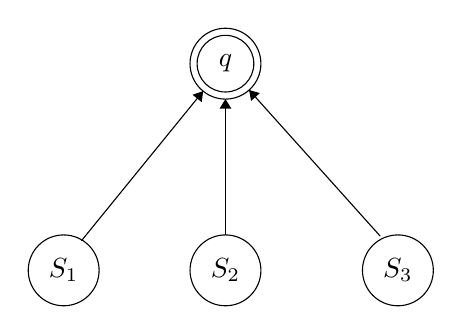
\begin{tikzpicture}[scale=0.15]
\tikzstyle{every node}+=[inner sep=0pt]
\draw [black] (37.7,-20.7) circle (3);
\draw (37.7,-20.7) node {$q$};
\draw [black] (37.7,-20.7) circle (2.4);
\draw [black] (24,-38.2) circle (3);
\draw (24,-38.2) node {$S_1$};
\draw [black] (52.3,-38.2) circle (3);
\draw (52.3,-38.2) node {$S_3$};
\draw [black] (37.7,-38.2) circle (3);
\draw (37.7,-38.2) node {$S_2$};
\draw [black] (25.5,-35.7) -- (35.81,-23.03);
\fill [black] (35.81,-23.03) -- (34.91,-23.33) -- (35.69,-23.96);
\draw [black] (37.7,-35.2) -- (37.7,-23.7);
\fill [black] (37.7,-23.7) -- (37.2,-24.5) -- (38.2,-24.5);
\draw [black] (50.8,-35.3) -- (39.7,-22.93);
\fill [black] (39.7,-22.93) -- (39.87,-23.86) -- (40.61,-23.19);
\end{tikzpicture}
\caption{An example of a Distributed Tracking instance on $h=3$ participants.}
\end{center}
\end{figure}


For illustrative purposes consider the following naive algorithm for the distributed tracking problem, where at each time step if a participants counter $c_i$ has been incremented, the corresponding participant $s_i$ reports it's new count to the coorindator. This clearly results in $O(\tau)$ messages over the course of the algorithm.

A more efficient algorithm, which we will make frequent use of in this thesis, is a result of Cormode \cite{Cormode2011}, though is presented (along with its proof) in a much more simplified manner.  
\begin{algorithm}
\caption{Efficient Distributed Tracking}\label{alg:dist-tracking}
\begin{algorithmic}[1]
\Procedure{DistributedTracking}{threshold $\tau$, participant set $S_1,\dots,S_h$}
\If{$\tau\leq6h$}
    \State \text{Commence brute-force algorithm by sending $O(\tau) = O(h)$ messages}
\EndIf
\State \text{Assign to each participant \textit{slack}} $\lambda \leftarrow \lfloor \tau/2h\rfloor$
\State \text{Assign to each participant $\bar{c}_i$ the value of $c_i$ the last time a signal was sent to $q$}
\For{\text{each timestamp}}
\If{$c_i - \bar{c}_i = \lambda$}
\State \text{participant $S_i$ transmits a signal to $q$}
\State $\bar{c}_i \gets c_i$
\EndIf
\State \text{after $q$ collects $h$ notifications set } $\tau^\prime\leftarrow\tau-\sum_{i=1}^{h}c_i$
\EndFor
\State \textbf{return} \text{DistributedTracking}$(\tau^\prime, S_1,\dots,S_h)$ \Comment{recursive call}
\EndProcedure
\end{algorithmic}
\end{algorithm}

\begin{theorem}[Correctness and Complexity]  For a participant set $S_1,\dots, S_h$ and threshold $\tau$ \cref{alg:dist-tracking} correctly reports the instant that $\sum_{i=1}^{h}c_i = \tau$. Moreover, the algorithm requires $O(h\log\tau)$ messages.
\end{theorem}
\begin{proof}
We begin by showing correctness. In the case that $\tau\leq6h$ correctness is trivial from using the brute force algorithm. To show correctness, we therefore must show that $\tau^\prime$ in line 12 is never negative. Observe that a transmission is sent every $\lambda$ counter increases, so 
\begin{align*}
    \sum_{i=1}^{h}c_i \leq h\lambda &= h \left\lfloor\frac{\tau}{2h} \right\rfloor \\
    &\leq \tau/2
\end{align*}
Thus in line 12 we have $\tau^\prime = \tau - \sum_{i=1}^{h}c_i\geq\tau/2 \geq 0$ concluding that the algorithm correctly reports maturation.

To analyse the efficiency of the algorithm, it is clear from lines 2 and 12 that each call to the procedure necessitates $\Omega(h)$ messages. We now bound the number of recursive calls which can be made via line 14. Let $T_h(\tau)$ denote the total messages sent for an instance of threshold $\tau$ and $h$ participants, our earlier analysis shows that at each recursive call, the threshold is reduced by a factor of at most $1/2$, leading to the recurrence relation
$$T_h(\tau) = T_h\left(\frac{\tau}{2}\right) + O(h)$$
It is rudimentary to show that this leads to a total of $O(\log\tau)$ recursive calls. Combined with the $\Omega(h)$ messages per call - this leads to a total of $O(h\log\tau)$ messages throughout the algorithm.
\end{proof}
